\documentclass{article}

\usepackage{arxiv}

\usepackage{hyperref}       % hyperlinks
\usepackage{url}            % simple URL typesetting
\usepackage{amsfonts}       % blackboard math symbols
\usepackage{amsmath}
\usepackage{nicefrac}       % compact symbols for 1/2, etc.
\usepackage{graphicx}
\usepackage{natbib}
\usepackage{csquotes}
\usepackage{float}
\usepackage{listings}
\usepackage{xcolor}
\usepackage{fancyvrb}

\definecolor{codegreen}{rgb}{0,0.6,0}
\definecolor{codegray}{rgb}{0.5,0.5,0.5}
\definecolor{codepurple}{rgb}{0.58,0,0.82}
\definecolor{backcolour}{rgb}{0.95,0.95,0.92}

\lstdefinestyle{mystyle}{
    backgroundcolor=\color{backcolour},
    commentstyle=\color{codegreen},
    keywordstyle=\color{magenta},
    numberstyle=\tiny\color{codegray},
    stringstyle=\color{codepurple},
    basicstyle=\ttfamily\footnotesize,
    breakatwhitespace=false,
    breaklines=true,
    captionpos=b,
    keepspaces=true,
    numbers=left,
    numbersep=5pt,
    showspaces=false,
    showstringspaces=false,
    showtabs=false,
    tabsize=2
}

\lstset{style=mystyle}


\title{Dark energy is based on a math error from 1930}

\date{\today}

\author{
  \href{https://orcid.org/0000-0001-6450-3262}{
\includegraphics[scale=0.06]{orcid.pdf}\hspace{1mm}Logan P.~Evans}
  \\ \texttt{loganpevans@gmail.com}
}

% Uncomment to override  the `A preprint' in the header
%\renewcommand{\headeright}{Technical Report}
%\renewcommand{\undertitle}{Technical Report}
\renewcommand{\shorttitle}{\textit{arXiv} Template}

\hypersetup{
pdftitle={Dark energy is based on a math error from 1930},
pdfsubject={astro-ph.CO},
pdfauthor={Logan P.~Evans},
pdfkeywords={cosmological parameters, dark energy},
}

\begin{document}
\maketitle

\begin{abstract}
  We show that the magnitude of distant objects has been calculated incorrectly
  since 1930. We describe how this math error has propagated for over nine
  decades. Finally, we explore the consequences of correcting this flaw and
  resolve two of the preeminent mysteries in cosmology: dark energy is not
  supported by observations of Type Ia supernovae, and the Hubble tension is
  due to a calculation error.
\end{abstract}

% keywords can be removed
\keywords{Cosmological Parameters \and Dark Energy \and Luminosity Distance \and Hubble tension}

\section{Introduction}

The measurement of Type Ia supernovae is one of the primary sources of data for
cosmological models. The measurements involve estimating the peak magnitude in
the B filter \citet{riess1998} for the rest frame, meaning we want to know how
bright the SnIa would be if its light didn't undergo redshift. Redshift causes
the light that would be mesaured by the B filter in a rest frame to be shifted
to another filter. In order to observe a SnIa in an arbitrary filter and report
the magnitude in the B filter we use a technique called K-corrections.

The first formal derivation of K-corrections was performed by
\citet{tolman1930}, and it failed to account for bandwidth stretching, one of
the dimming effects of redshift. This error was noted by \citet{desitter1934},
but in \citet{hubble1935} the descrepancy was noted and ignored.
\citet{oke1968} rederived K-corrections, but they failed to account for time
dilation, one of the other dimming effects of redshift. In \citet{kim1996},
K-corrections were extended to handle additional cross-filter comparisons and
address zero-point corrections, but they started their derivation by
referencing the incorrect equation from \citet{oke1968}. \citet{hsiao2007}
expanded on the work done by \citet{kim1996} by providing expected SnIa
template spectra. Finally, \citet{burns2010} implemented the popular software
package Sn(OO)py which implemented the SnIa template spectra into
K-corrections. This software package computes K-corrections differently from
prior work, and in order to match prior values, the code adds an extra term.
This history is explored in more depth in Section \ref{sec:history}.

The effect of using an incorrect magnitude for SnIa is that we think objects
are farther away than they really are, and the effect componds for greater
distances. Up until \citet{riess1998}, we didn't have distant enough
observations for this error to matter much for cosmology models, but in the
late 1990s, it was clear that our measurements for distance and redshift were
not linear. This observation led to a model that utilized a cosmological
constant and dark energy in order to explain the non-linear distance-redshift
graph. We will show in Section \ref{sec:correction} that correcting the flaw
with K-corrections leads to a linear graph that does not need to rely on a
cosmological constant.

Since \citet{planck2020}, it has been evident that something was missing with
our understanding of cosmology. This research used an alternative technique
based on measurements of the cosmic microwave background to measure the Hubble
constant, but as summarized in \citet{perivolaropoulos2022}, this measurement
was incompatable with the Hubble constant measured from SnIa. As we will
discuss in Section \ref{sec:tension}, fixing the error with K-corrections
produces a measurement of the Hubble constant that is compatible with models
based on the cosmic microwave background.

\section{A brief history of K-corrections}
\label{sec:history}

Observations of Type Ia supernova are essential to calibrate models that
measure redshift and estimate distance. This relationship, often called the
Hubble-Lema\^{i}tre law, describes how quickly the universe is expanding.
However, \citet{riess1998} and \citet{perlmutter1999} presented evidence that
there isn't a linear relationship between redshift and distance, but instead,
distant objects are farther away than their redshift would predict (see Figure
\ref{fig:mu_distance_vs_redshift}). This phenomenon implies that the
acceleration of the universe is faster today than it was for old observations.
Previously the cause of this phenomenon was unknown and was referred to as
dark energy.

\begin{figure}[h]
  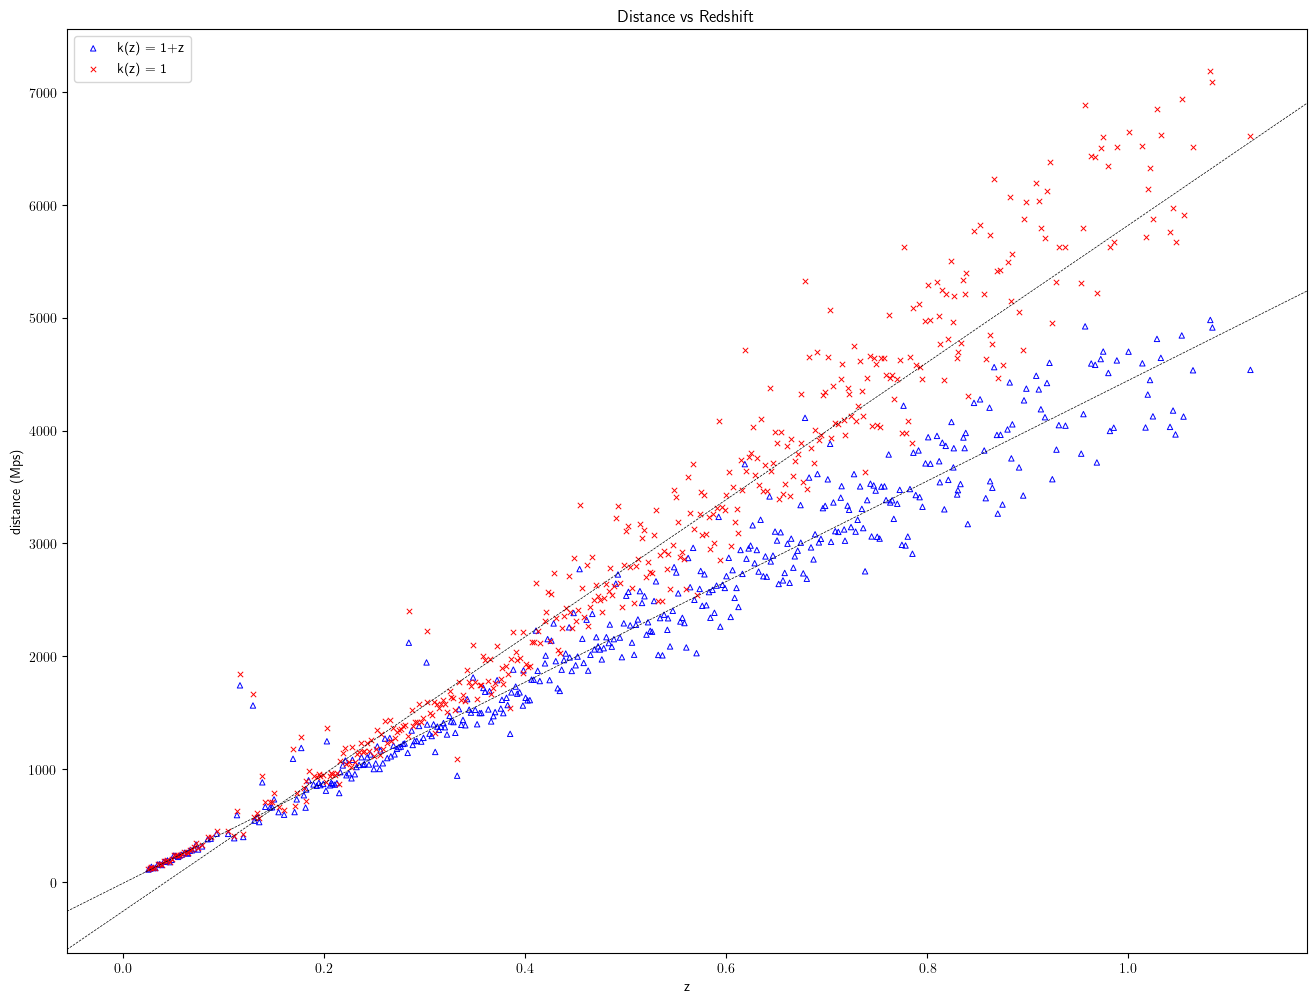
\includegraphics[width=\linewidth]{mu_distance_vs_redshift.png}
  \caption{The relationship between distance and redshift for two treatments of
  magnitude data. The displayed points are roughly a third of the values in the
  full DES dataset, selected evenly to aid visibility. The $k(z) = 1$ treatment
  is clearly non-linear while the $k(z) = 1 + z$ treatment appears to be
  linear.}
  \label{fig:mu_distance_vs_redshift}
\end{figure}

Type Ia supernova are used to explore the relationship between distances and
redshifts because these events always happen in similar ways, so the absolute
brightness is roughly always the same. An analogy is to imagine someone walking
in the dark and lighting matches. As long as we know how brightly a match burns
at a known distance, we can estimate the distance to any match by measuring the
appearant brightness before applying some geometry.

Measuring the apperant brightness of a Type Ia supernova is non-trivial. The
aspect of the process that we will explore here concerns how redshift affects
the light we observe. This problem is often referred to as K-corrections, and
one of the first mathematical treatments of the problem was performed by
\citet{tolman1930}. However, when Tolman made his derivation, he did not
consider the effects of a spectra that is stretched out due to redshift.

A few years later, \citet{desitter1934}, discussed all three issues that reduce
the observed magnitude of a distant observation. The correction for each of
these issues is identical: take a measurement for luminosity and multiply it by
the factor $1 + z$.

A year later, \citet{hubble1935} published a similar set of calculations for
K-corrections, but these equations used $(1 + z)^2$ instead of the $(1 + z)^3$
correction term used by de Sitter. They started their derivation by copying the
incorrect equation from 1930. After their derivation, they noted,

\begin{quote}
It should be specially noted that this expression differs from the correction
to m proposed by de Sitter, which contains the term $(1 + z)^3$ instead of
$(1 + z)^2$. Expression (28), however, would seem to give the proper correction
to use in connection with our equation (21), since it has been derived in such
a way as to make appropriate allowance, first, for the double effect of nebular
recession in reducing both the individual energy and the rate of arrival of
photons, and then for the further circumstance that a change in spectral
distribution of the energy that does arrive will lead to changes in its
photographic effectiveness.
\end{quote}

The Hubble K-corrections with the incorrect correction term have been used ever
since.

By \citet{oke1968}, the two factors of $(1 + z)$ were attributed to the change
in energy and to the spectral bandwidth elongation, which leaves time dilation
as the factor that was omitted. A graph that demonstrates why it's essential to
correct for both the spectra bandwidth warping and time dilation is presented
in Figure \ref{fig:k-example}.

\begin{figure}[H]
  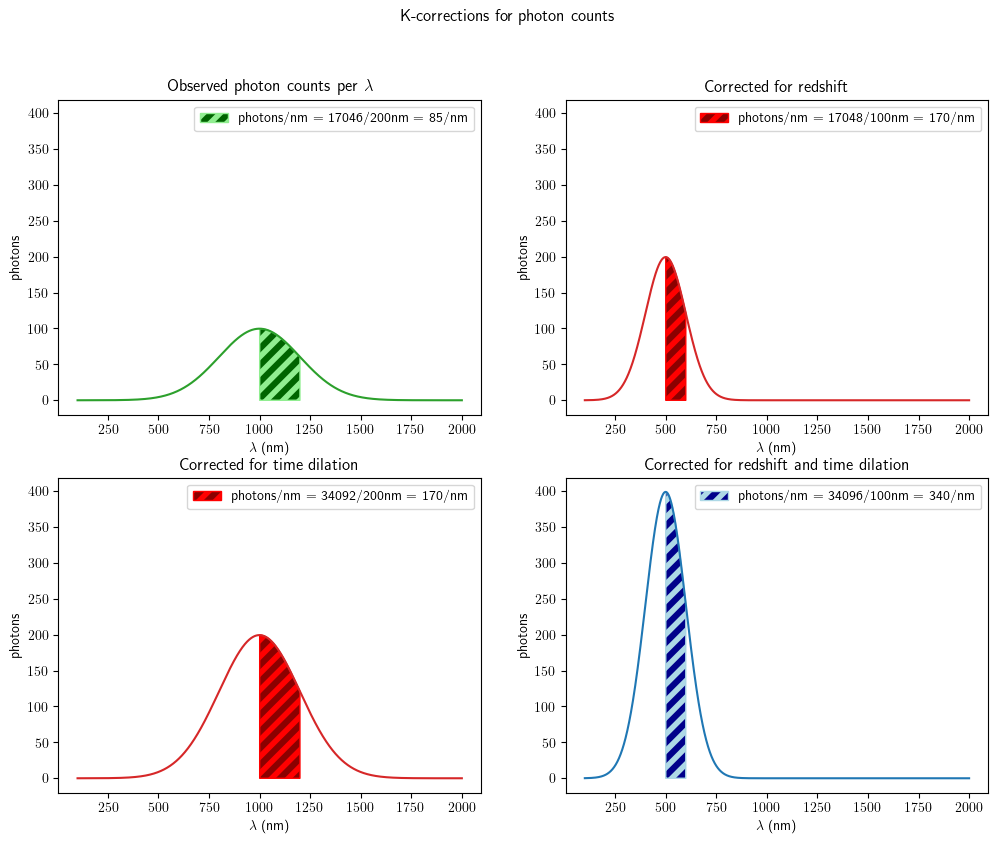
\includegraphics[width=.75\linewidth]{K-corrections_for_photon_counts.png}
  \caption{An example of how K-corrections take an observed magnitude and
  produce a rest frame magnitude. In this example, $z=1$. The observation
  filter measures magnitude, which is equivalent to measuring the number of
  photons per nanometer. In the bottom left panel, a correction of $1+z$ is
  applied which doubles the photons per nanometer. The top right panel shows
  the effect of correcting for the bandwidth spectrum warping effect --
  correcting all wavelengths for the rest frame means that the measured
  wavelengths have blueshifted, ideally into the cross band B filter. Applying
  both effects, shown in the bottom right panel, requires applying two
  correction factors of $1+z$. This example omits the correction for a similar
  effect related to lower energy due to the Planck relation because CCD cameras
  obviate the need to correct for this effect.
  }
  \label{fig:k-example}
\end{figure}

The modern treatment of K-corrections is based on the work of \citet{kim1996}.
This work extended the calculations of K-corrections to extend to filters
beyond B and V. It also introduced a term that deals with the zero-point for
the actual filters. In the modern day, filters measure the photon flux as
upposed to the energy flux. Historically, bolometric devices would measure the
energy flux, but modern CCD cameras effectively measure the photon flux.

Quoting \citet{kim1996}:

\begin{quote}
  Therefore, the correct K correction caluculation to be used with measured
  photometric magnitudes is the integral photon counts:

  \begin{equation}
  \label{eq:kim}
    K_{xy} =
      -2.5\text{log} \left(
        \frac{\int \lambda \mathcal{Z}(\lambda)S_x(\lambda)d\lambda}
             {\int \lambda \mathcal{Z}(\lambda)S_y(\lambda)d\lambda}\right)
      + 2.5\text{log}(1+z)
      + 2.5\text{log}\left(
        \frac{\int \lambda F(\lambda)S_x(\lambda)d\lambda}
             {\int \lambda F(\lambda/(1+z))S_y(\lambda))d\lambda}\right).
  \end{equation}
\end{quote}

This equation has three errors, which we will explore in Section
\ref{sec:consequences}.

\section{Derivation of K-corrections}
\label{sec:derivation}

With modern CCD cameras, a telescope observaion consists of a single value
$\mathcal{F}_x$ erg/s, which represents the energy collected in filter $x$ per
second. A summary of how this works is provided by \citet{lesser2015}. The
measured energy is produced by electrons not photons, so the measured number is
proportional to the number of photons. However, we need to calculate the
expected number of photons collected by using a spectral energy density
function $F$. The value $F(\lambda)$ gives the amount of energy collected by a
bolometric device for the wavelength $\lambda$.

To convert the spectral energy density $F$ to the photon density $F'$, we need
to use the Plank relation $E = \frac{hc}{\lambda}$ where $E$ is the energy, $h$
is Planck's constant, and $c$ is the speed of light. This gives us

\begin{equation}
\begin{aligned}
   F(\lambda) &= F'(\lambda) \times \frac{hc}{\lambda} \\
  F'(\lambda) &= \frac{\lambda F(\lambda)}{hc}.
\end{aligned}
\end{equation}

It's important to note that for the blueshifted wavelength $\lambda / (1+z)$,
this equation produces

\begin{equation}
 F'\left(\frac{\lambda}{1+z}\right) = \frac{\left(\frac{\lambda}{1 + z}\right) F\left(\frac{\lambda}{1+z}\right)}{hc}.
\end{equation}

However, this equation is misleading and error prone. We will want to use it to
help calculate the amount of flux in an observation filter at the redshifted
wavelength $\lambda \times (1 + z)$. In other words, we want to produce the
photon density function $R'$ that is the redshifted version of $F'$.
Redshifting does two things:

\begin{itemize}
  \item The stretching of space increases the distance between photons while
  they are traveling. This phenomenon appears to an observer like time
  dilation, although cosmological time dilation is due to a different mechanism
  than relativistic time dilation. This effect reduces the photon arrival rate
  by a factor of $1/(1+z)$.

  In order to account for cosmological time dilation, we will need to multiply
  $F'$ by $1/(1+z)$.

  \item All wavelengths are changed by a factor of $1 + z$. When we integrate
  $R'$ from wavelength $\lambda_a$ to wavelength $\lambda_b$, the values
  correspond to the wavelengths $\lambda_a / (1+z)$ to $\lambda_b / (1+z)$ in
  $F'$. We will integrate over a width of $\lambda_b - \lambda_a$, but
  $F'(\lambda / (1+z))$ will refer to values in a width of
  $(\lambda_b - \lambda_a) / (1+z)$.

  In order to account for this bandwidth spectral warping effect, we will need
  to multiply $F'$ by a second factor of $1/(1+z)$.
\end{itemize}

Combining these two phenomena together, we can calculated the redshifted
spectral energy density $R$ using

\begin{equation}
\begin{aligned}
\label{eq:redshifted_density}
  R'(\lambda) &= F'(\lambda / (1+z)) \times \frac{1}{(1 + z)^2} \\
  R(\lambda) &= \frac{F(\lambda / (1+z))}{(1+z)hc} \times \frac{1}{(1 + z)^2} .
\end{aligned}
\end{equation}

In order to calculate the amount of flux $\mathcal{F}_x$ measured in filter
$x$, we need to compute the photon density $F'(\lambda)$ and multiply it by
sensity $S_x(\lambda)$, which represents the proportion of photons filter $x$
will measure at wavelength $\lambda$. We then need to sum over all wavelengths,
which is expressed with the equation

\begin{equation}
\begin{aligned}
\label{eq:flux_definition}
  \mathcal{F}_x &= \int F'(\lambda) S_x(\lambda) d\lambda \\
                &= \int \lambda F(\lambda) S_x(\lambda) d\lambda.
\end{aligned}
\end{equation}

The limits of integration are techinically from 0 to $\infty$, but these are
usually not written because the sensitivity $S(\lambda)$ is 0 for wavelengths
outside of a filter's bandpass.

We will also use the energy flux $\mathcal{F}$ to magnitude $m$ formula:

\begin{equation}
\begin{aligned}
\label{eq:flux2mag}
                             m_x &= -2.5 \text{log}(\mathcal{F}_x) + P_x \\
  -2.5 \text{log}(\mathcal{F}_x) &= m_x - P_x .
\end{aligned}
\end{equation}

$P_x$ represents the zero-point for the filter $x$ on some particular
telescope. In order to use consistant magnitude values across telescopes that
have different light gathering abilities, we take the measured magnitude and
multiply it by the ratio of the standard flux rate to the flux rate for this
particular telescope and filter. For convenience, we use $P_x = -2.5
\text{log}(P'_x)$ so that we can work with flux instead of with magnitude.

Now that we have the identities in Equations \ref{eq:flux_definition} and
\ref{eq:flux2mag} we will change directions and look at the definition of
K-corrections $K_{xy}$. This value allows us to make an observation in filter
$y$ and report what the magnitude would have been in filter $x$ if no redshift
occured:

\begin{equation}
\begin{aligned}
\label{eq:definition}
  m_y &= M_x + \mu + K_{xy} \\
      &= M_x + m_x - M_x + K_{xy} \\
      &= m_x + K_{xy} \\
  m_x &= m_y - K_{xy} .
\end{aligned}
\end{equation}

The second line of Equation \ref{eq:definition} expands the distance modulus
$\mu$ using $\mu = m - M$ where $m$ is the observed magnitude and $M$ is the
absolute magnitude.

Since the K-correction is a magnitude value and we wish to work on flux values,
it is convenient to define the following substitution:

\begin{equation}
\label{eq:k_substitution}
  K_{xy} = 2.5\text{log}(K'_{xy}) .
\end{equation}

Note that this substitution omits the minus ($-$) sign.

Starting with Equation \ref{eq:flux2mag} and then
recombining the flux term $\mathcal{F}_y$ with $m_y$ from Equation
\ref{eq:definition}, we have

\begin{equation}
\begin{aligned}
\label{eq:as_flux}
  -2.5 \text{log}(\mathcal{F}_x)
      &= m_x - P_x \\
      &= m_y - K_{xy} - P_x \\
      &= -2.5 \text{log}(\mathcal{F}_y) + P_y - K_{xy} - P_x \\
      &= -2.5 \text{log}(\mathcal{F}_y)
         - 2.5 \text{log}(P'_y)
         - 2.5 \text{log}(K'_{xy})
         + 2.5 \text{log}(P_x) \\
      &= -2.5 \left(
         \text{log}(\mathcal{F}_y)
         + \text{log}(K'_{xy})
         + \text{log}(P'_y)
         - \text{log}(P'_x)
        \right) \\
      &= -2.5 \text{log}\left(
        \mathcal{F}_y
        \times K'_{xy}
        \times \frac{P'_y}{P'_x}\right) \\
  \mathcal{F}_x &= \mathcal{F}_y \times K'_{xy} \times \frac{P'_y}{P'_x}.
\end{aligned}
\end{equation}

It's useful to inspect this equation to consider whether the term
$\frac{P'_y}{P'_x}$ is correct, or if it might be flipped to the inverse of
what it should be. However, if we rewrite Equation \ref{eq:as_flux} as

\begin{equation}
  \mathcal{F}_x \times P'_x = \mathcal{F}_y \times P'_y \times K'_{xy}
\end{equation}

then the meaning is a bit more clear. The left hand side
$\mathcal{F}_x \times P'_x$ is the rate of photon collection for an idealized
telescope in filter $x$ while $\mathcal{F}_y \times P'_y$ is the rate of photon
collection for an idealized telescope in filter $y$. We are able to observe the
value $\mathcal{F}_y \times P'_y$ and want to use the fudge factor $K'_{xy}$ to
produce the value $\mathcal{F}_x \times P'_x$.

We can isolate $K'_{xy}$ and then use Equation \ref{eq:flux_definition} to expand

\begin{equation}
\begin{aligned}
  \mathcal{F}_x &= \mathcal{F}_y \times K'_{xy} \times \frac{P'_y}{P'_x} \\
        K'_{xy} &= \frac{\mathcal{F}_x P'_x}{\mathcal{F}_y P'_y} .
\end{aligned}
\end{equation}

Now we use Equations \ref{eq:redshifted_density} and \ref{eq:flux_definition}
to calculate the fluxes $\mathcal{F}_x$ and $\mathcal{F}_y$ in terms of the
spectral energy density function $F$. Note that $\mathcal{F}_x$ uses the rest
frame spectral energy density $F$ while $\mathcal{F}_y$ uses the redshifted
spectral energy density $R(\lambda)$:

\begin{equation}
\begin{aligned}
  K'_{xy} &= \frac{\mathcal{F}_x P'_x}{\mathcal{F}_y P'_y} \\
         &= \frac{P'_x \int F'(\lambda) S_x d\lambda}
                 {P'_y \int R'(\lambda) S_y d\lambda} \\
         &= \frac{P'_x}{P'_y} \times
              \frac{\int F'(\lambda) S_x d\lambda}
                   {\int F'(\lambda / (1+z)) \times \frac{1}{(1 + z)^2} d\lambda} \\
         &= \frac{P'_x}{P'_y} \times (1+z)^2 \times
              \frac{\int \frac{\lambda F(\lambda)}{hc} S_x d\lambda}
                   {\int \frac{F(\lambda / (1+z))}{(1+z)hc} S_y d\lambda} \\
         &= \frac{P'_x}{P'_y} \times (1 + z)^2 \times
              \frac{\int \lambda F(\lambda) S_x d\lambda}
                   {\int \frac{\lambda}{1+z} F(\lambda / (1+z)) S_y d\lambda} .
\end{aligned}
\end{equation}

Finally, we can use Equation \ref{eq:k_substitution} to convert the flux $K'_{xy}$ back
into the magnitude $K_{xy}$:

\begin{equation}
\begin{aligned}
\label{eq:K2k}
  K_{xy} &= 2.5\text{log}(K'_{xy}) \\
         &= 2.5\text{log}\left(
            \frac{P'_x}{P'_y} \times (1 + z)^2 \times
            \frac{\int \lambda F(\lambda) S_x d\lambda}
                 {\int \frac{\lambda}{1+z} F(\lambda / (1+z)) S_y d\lambda}\right) \\
         &= 2.5 \left(
            \text{log} \left( \frac{P'_x}{P'_y} \right)
            + \text{log}( {(1 + z)^2})
            + \text{log}\left( \frac{\int \lambda F(\lambda) S_x d\lambda}
                   {\int \frac{\lambda}{1+z} F(\lambda / (1+z)) S_y d\lambda}
            \right) \right) \\
         &= 2.5 \text{log} \left( \frac{P'_x}{P'_y} \right)
            + 5 \text{log} (1 + z)
            + 2.5 \text{log} \left(
              \frac{\int \lambda F(\lambda) S_x d\lambda}
                   {\int \frac{\lambda}{1+z} F(\lambda / (1+z)) S_y d\lambda} \right) \\
         &= 5 \text{log} (1 + z)
            + 2.5 \text{log} \left(
              \frac{\int \lambda F(\lambda) S_x d\lambda}
                   {\int \frac{\lambda}{1+z} F(\lambda / (1+z)) S_y d\lambda} \right)
            - P_x + P_y .
\end{aligned}
\end{equation}

\section{Consequences}
\label{sec:consequences}

In order to fully compare our derivation against Equation \ref{eq:kim}, we need
to use the identity

\begin{equation}
  P = -2.5 \text{log} \left( \int \mathcal{Z}(\lambda) S_x(\lambda) d\lambda \right)
\end{equation}

where, according to \citet{kim1996}, "$\mathcal{Z}(\lambda)$ is an idealized
spectral energy distribution at $z = 0$ for which $U = B = V = R = I = 0$ in
the photometric system being used." Combining this with Equation \ref{eq:K2k}, we have

\begin{equation}
\begin{aligned}
  K_{xy} &= 5 \text{log} (1 + z)
            + 2.5 \text{log} \left(
              \frac{\int \lambda F(\lambda) S_x d\lambda}
                   {\int \frac{\lambda}{1+z} F(\lambda / (1+z)) S_y d\lambda} \right)
            - P_x + P_y \\
         &= 5 \text{log} (1 + z)
            + 2.5 \text{log} \left(
              \frac{\int \lambda F(\lambda) S_x d\lambda}
                   {\int \frac{\lambda}{1+z} F(\lambda / (1+z)) S_y d\lambda} \right)
            + 2.5 \text{log} \left( \int \mathcal{Z}(\lambda) S_x(\lambda) d\lambda \right)
            - 2.5 \text{log} \left( \int \mathcal{Z}(\lambda) S_y(\lambda) d\lambda \right) \\
         &= 2.5 \text{log} \left(
              \frac{\int \mathcal{Z}(\lambda) S_x(\lambda) d\lambda}
                   {\int \mathcal{Z}(\lambda) S_y(\lambda) d\lambda}
             \right)
            + 5 \text{log} (1 + z)
            + 2.5 \text{log} \left(
              \frac{\int \lambda F(\lambda) S_x d\lambda}
                   {\int \frac{\lambda}{1+z} F(\lambda / (1+z)) S_y d\lambda} \right) .
\end{aligned}
\end{equation}

\begin{minipage}[c]{0.95\textwidth}
\lstinputlisting[language=Python, caption=A demonstration that K-corrections
calculated by snpy are off by \texttt{2.5*log10(1+z)}. The roundoff error is
roughly \texttt{2e-16}.]{code_listing.py}
\end{minipage}

\section{The dimming effects of redshift}
\label{sec:redshift}

The magnitude measurements for Type Ia supernova goes through a long chain of
data processing. The data used here was collected by the Dark Energy Survey
Collaboration, as summarized in \citet{abbott2024} and described in more detail
by \citet{vincenzi2024}. However, the data processing does not explicitly
correct for either redshift or time dilation.

In the big bang model, there are multiple phenomena associated with redshift that we
might expect to reduce the apparent magnitude of a Type Ia supernova.

\subsection{Recessional velocity redshift}

The energy carried by a photon is inversely proportional to wavelength, given
by the Planck relation

\begin{equation}
  E = \frac{hc}{\lambda}
\end{equation}

where $E$ is energy, $h$ is the Planck constant, $c$ is the speed of light, and
$\lambda$ is the wavelength.

As redshift increases the wavelength of a photon, the energy decreases.

The supernova data collected by the DES Collaboration used a CCD camera, a
photon counting device, as described by \citet{flaugher2015}.  \citet{kim1996}
noted that photometric measurements that depend on bolometers will need to be
corrected for the reduced energy level of redshifted light, but with a photon
counting device, this correction is not necessary.

While the redshift phenomenon should impact the light detected from distant
supernova, it should not impact the magnitude measurements so it does not need
to be explicitly corrected.

\subsection{Time dilation}

The second phenomenon is that time dilation for objects moving quickly relative
to our observational rest frame will reduce the rate at which photons are being
emitted. Instead of changing the properties of individual photons, time
dilation reduces the count of photons by a factor of $\frac{1}{1+z}$ where $z$
is the redshift.

This phenomenon will not be addressed by the nuances of any measuring device,
so it must be explicitly corrected.

\subsection{Stretching of space}

If space itself is stretching, it will both increase the wavelength of photons
and also reduce the density of those photons. If space is stretching at a
constant rate, the effect would be indistinguishable from the redshift and time
dilation created by high relative recessional velocities. However, an
accelerating expansion of the universe may indicate a non-constant rate of
stretching. This would manifest by distant objects having a greater distance
per redshift than nearby objects.

This non-linear streching-of-space model would be indistinguishable from a
scenario where a constant force is pushing all objects away from each other.

\subsection{Tired light}

An alternative to the big bang theory is the tired light hypothesis, as
described by \citet{zwicky1929} and \citet{shao2013}. The idea is that distant
objects are mostly stationary relative to us, but the energy of light is lost
as it travels through space. A feature of the tired light hypothesis is that
since distant objects do not have a high relative velocity to us, they should
not show time dilation.

However, as shown by \citet{blondin2008} and \citet{white2024}, distant
supernova do experience time dilation. Based on this, we can reject the tired
light hypothesis and assume the big bang model.

\section{Correcting magnitude for time dilation}
\label{sec:correction}

Luminosity distance $D_L$, is the apparent distance of an object based on the
observed luminosity, also known as the flux $F$. This does not take into
account any movement of the observed object between the time when the light was
emitted and the light is observed.

To derive the luminosity distance from these measurements, we start
by computing the flux $F$. Magnitude $m$ is defined on a logarithmic scale
where magnitude 1 has 100 times the brightness of magnitude 6, leading to

\begin{equation}
  F = \frac{1}{\sqrt[5]{100}^{m - 1}}.
\end{equation}

This is proportional to the number of photons detected by a telescope. We can
find the corrected flux $F^*$ by multiplying by $k(z)$, the redshift correction
factor. Time dilation of quickly moving objects reduces the number of photons
by a factor of $\frac{1}{1 + z}$, so we have

\begin{equation}
\begin{aligned}
  F^* &= F \times k(z) \\
      &= F (1 + z).
\end{aligned}
\end{equation}

To compute the corrected magnitude $m^*$, we can solve

\begin{equation}
\begin{aligned}
   F^* &= \frac{1}{\sqrt[5]{100}^{m^* - 1}} \\
   m^* &= m - \frac{\ln{(z + 1)}}{\ln{(\sqrt[5]{100})}}.
\end{aligned}
\end{equation}

From here, we can use the standard distance modules $\mu$ defined as

\begin{equation}
  \mu = m^* - M
\end{equation}

where $M$ is the absolute magnitude. The luminosity distance $D_L$ in parsecs
can then be calculated as

\begin{equation}
  D_L = 10^{1 + \frac{\mu}{5}}.
\end{equation}

\section{Linear distance vs redshift relationship}
\label{hubblelaw}

The theory of an accelerating expansion is based on there being a non-linear
relationship between redshift and distance. More specifically, old objects (the
ones that are more distant) should have more distance per redshift than newer
objects.

As shown in Figure \ref{fig:mu_distance_vs_redshift}, this non-linear
relationship is only observed when $k(z) = 1$, meaning that magnitude is not
corrected for time dilation.

In contrast, when $k(z) = 1 + z$, time dilation is accounted for and there is a
linear relationship between redshift and distance. A linear model rules out an
accelerated expansion.

\begin{figure}[ht]
  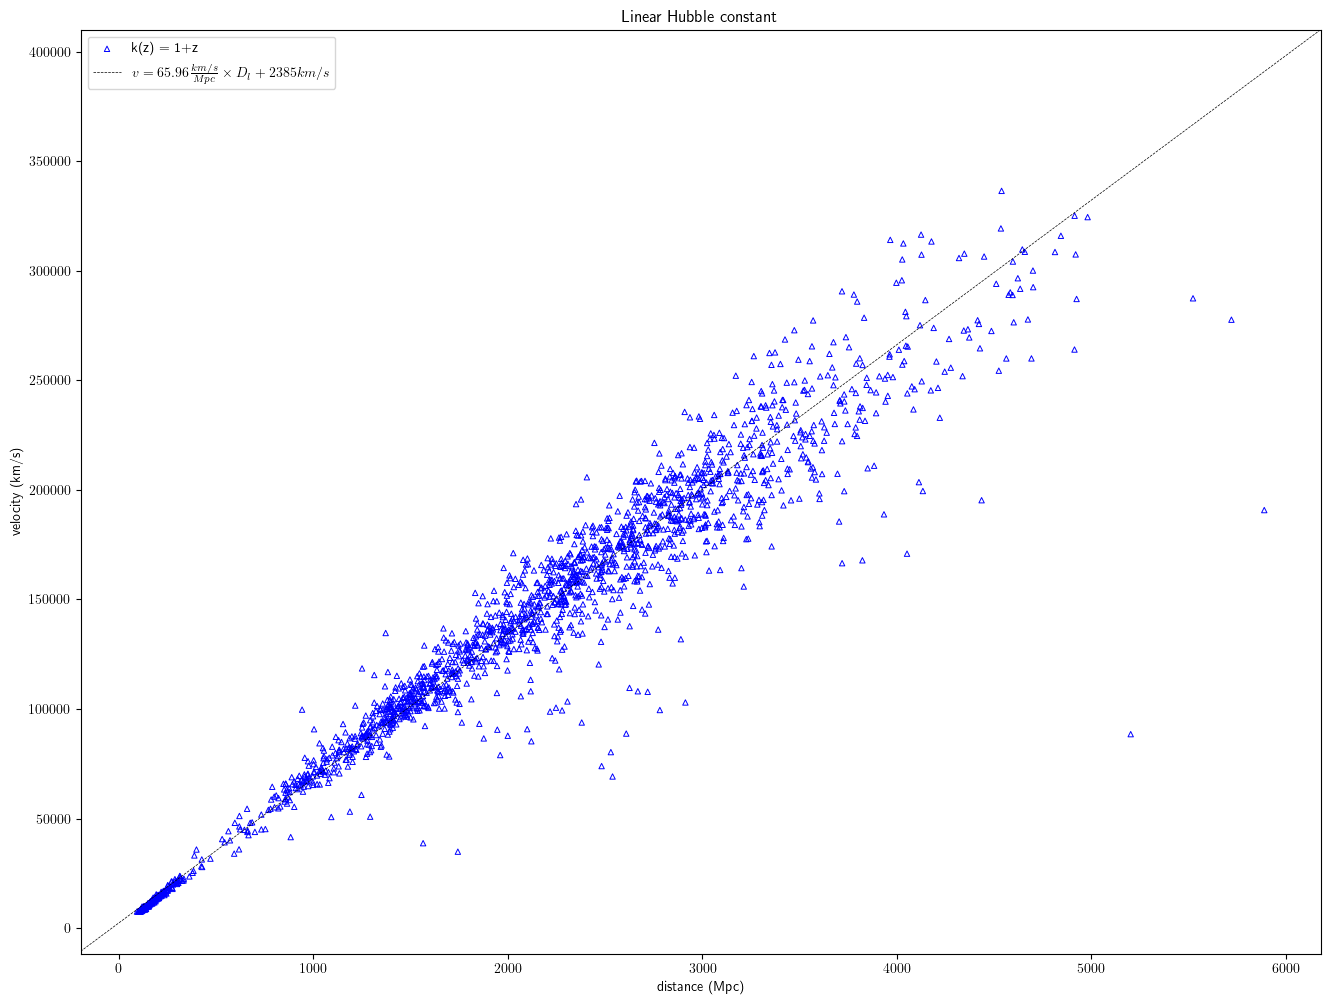
\includegraphics[width=\linewidth]{velocity_vs_distance.png}
  \caption{The relationship between expansion velocity and distance. The slope of this graph demonstrates the Hubble constant.
  }
\end{figure}

\section{Hubble tension}
\label{sec:tension}

\begin{figure}[ht]
  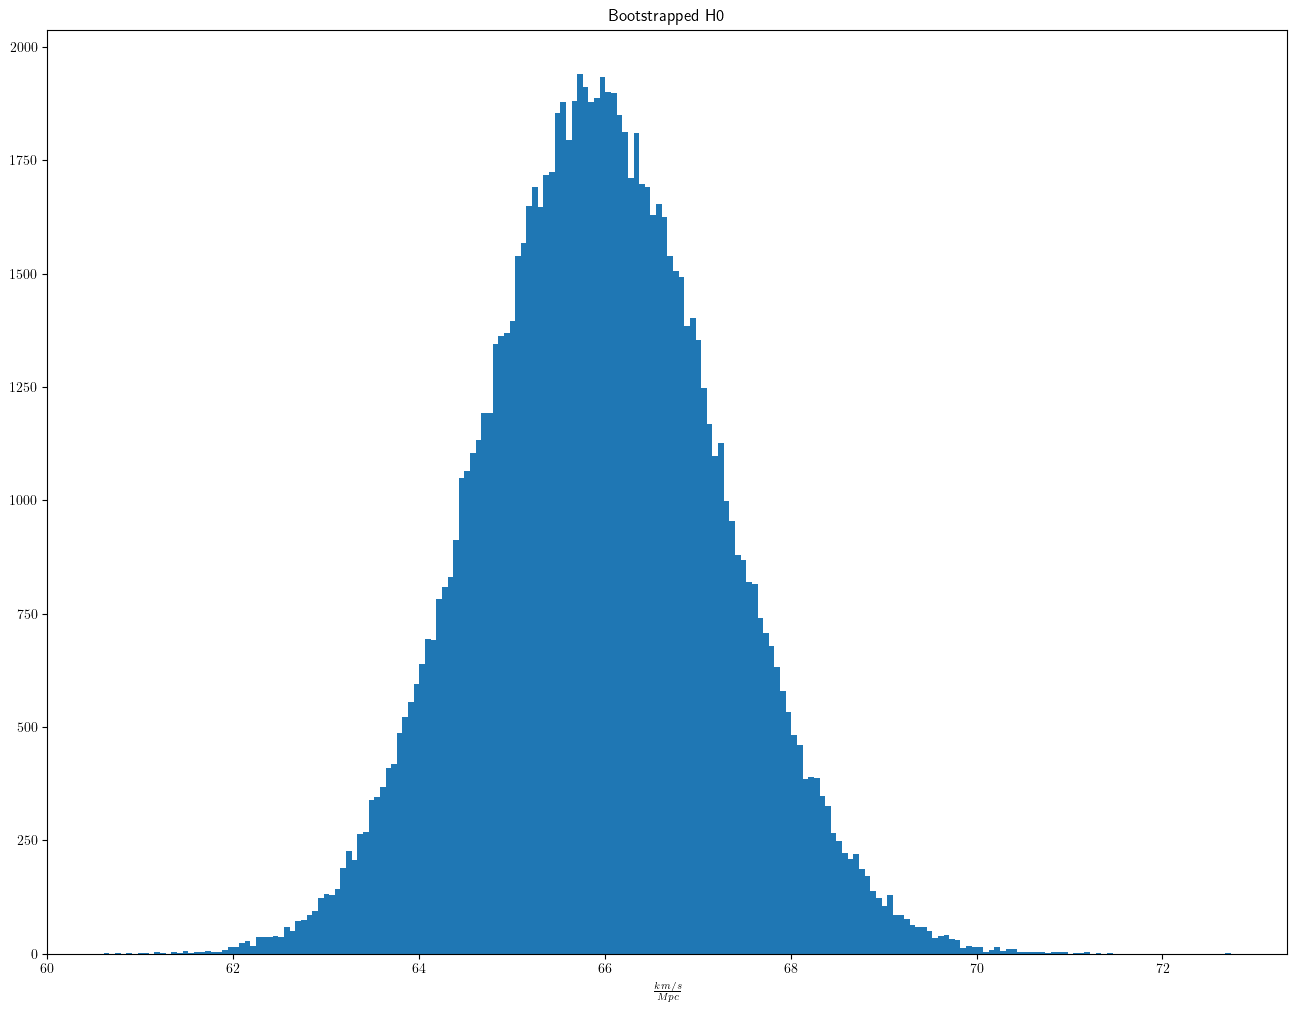
\includegraphics[width=\linewidth]{bootstrapped_H0.png}
  \caption{A histogram of 100000 bootstrap trials measuring the Hubble constant
  $H0$. Each trial samples an absolute Type Ia magnitude $M \sim Norm(-19.2334,
  0.0404)$ based on data published by \citet{camarena2020}. It then samples,
  with replacement, a population of supernovae from the dataset published by
  \citet{abbott2024}. Finally, it uses the non-parametric linear regression
  technique described by \citet{siegel1982}. The result of the bootstrap is $H0
  \sim Norm(65.94, 1.29)$.
  }
\end{figure}

Previous studies use $F$ instead of $F*$. To the best of our knowledge, no
studies that depend on the distance of Type Ia supernova, reaching back at
least to \citet{kim1996}, \citet{riess1998}, and \citet{perlmutter1999}, have
accounted for time dilation.

\bibliographystyle{unsrtnat}
\bibliography{references}

\end{document}
